%
% $Id$
% 
%       This source code is part of
% 
%        G   R   O   M   A   C   S
% 
% GROningen MAchine for Chemical Simulations
% 
%               VERSION 2.0
% 
% Copyright (c) 1991-1999
% BIOSON Research Institute, Dept. of Biophysical Chemistry
% University of Groningen, The Netherlands
% 
% Please refer to:
% GROMACS: A message-passing parallel molecular dynamics implementation
% H.J.C. Berendsen, D. van der Spoel and R. van Drunen
% Comp. Phys. Comm. 91, 43-56 (1995)
% 
% Also check out our WWW page:
% http://md.chem.rug.nl/~gmx
% or e-mail to:
% gromacs@chem.rug.nl
% 
% And Hey:
% Giving Russians Opium May Alter Current Situation
%

\chapter{Special Topics}
\label{ch:special}
\section{Calculating potentials of mean force: the pull code}
\label{sec:pull}
There are a number of options to calculate \swapindex{potentials
of}{mean force}\index{force, potential of mean|see{potentials of mean force}}
\index{free energy calculations}
and related topics. In the current version of {\gromacs} this is
implemented through some extra files for {\tt mdrun}. 

\subsection{Overview}
Four different types of calculation are supported:

\begin{enumerate}
\item{\textbf{Constraint forces}} The distance between the centers of
mass of two groups of atoms can be constrained and the 
\swapindex{constraint}{force} monitored.
The distance can be in 1, 2, or 3 dimensions. This method
uses the SHAKE algorithm but only needs 1 iteration to be
exact if only two groups are constrained. 
\item{\textbf{Umbrella sampling}} A simple
\swapindex{umbrella}{sampling} with an
harmonic umbrella potential that acts on the center of mass of a group
of atoms.
\item{\textbf{\swapindex{AFM}{pulling}}} A spring is connected to an atom and
slowly retracted. This has the effect of pulling an atom or group of
atoms away from its initial location. The rate constant and spring
constant for the spring can be varied to study e.g. the unbinding of a
protein and a ligand (see figure~\ref{fi:pull}). 
\begin{figure}
\centerline{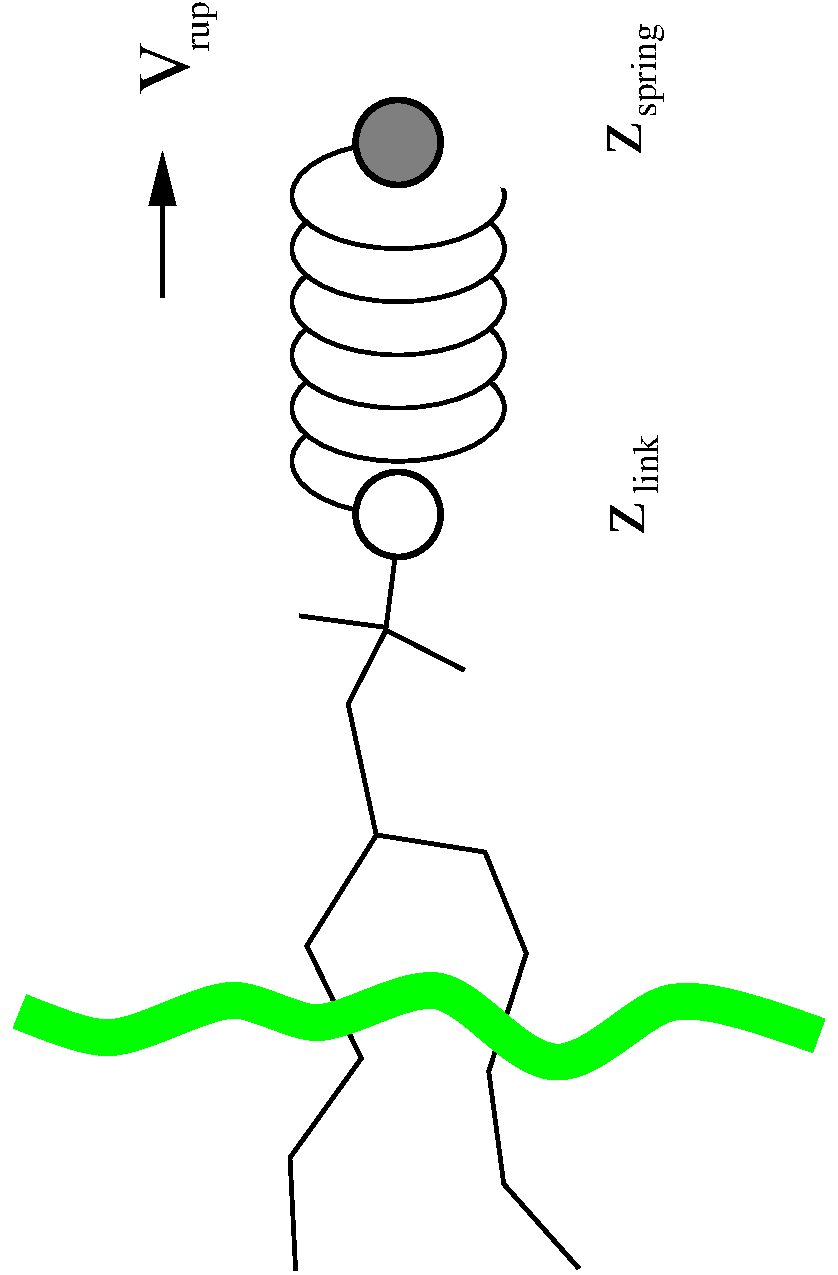
\includegraphics[width=6cm,angle=270]{plots/pull}}
\caption{Schematic picture of pulling a lipid out of a lipid bilayer
with AFM pulling. $V_{rup}$ is the velocity at which the spring is
retracted, $Z_{link}$ is the atom to which the spring is attached and
$Z_{spring}$ is the location of the spring.}
\label{fi:pull} 
\end{figure}   
\item{\textbf{Starting structures}} This option creates a number of
starting structures for potential of mean force calculations, moving 1
or 2 groups of atoms at a specified rate towards or away from a
reference group, writing out a coordinate file at specified intervals.
Note that the groups given in the index file are translated a
specified distance each step, but in addition also undergo the normal
MD, subject to definitions of \emph{e.g.} temperature coupling groups, freeze
groups and the like.
\end{enumerate}

In the calculations, there has to be 1 reference group and 1 or 2
other groups of atoms. For constrained runs, the distance between the
reference group and the other groups is kept constant at the distance
they have in the input coordinate file ({\tt .tpr}) file.

\subsection{Usage}

\subsubsection{Input files}

The {\tt mdrun} programs needs 4 additional files: 2 input files and 2
output files. 
\begin{description}
\item[\tt -pi pull.ppa]\mbox{}\\ If this file is specified the pull code will
be used. It contains the parameters that control what type of
calculation is done. A full explanation of all the options is given below.
\item[\tt -pn index.ndx]\mbox{}\\ This file defines the different groups for
use in all pull calculations. The groups are referred to by name, so
the index file can contain other groups that are not used as well. 
\item[\tt -po pullout.ppa]\mbox{}\\ A formatted copy of the input parameter
file with the parameters that were actually used in the run.
\item[\tt -pdo pull.pdo]\mbox{}\\ The data file with the calculated forces
(AFM pulling, constraint force) or positions (umbrella sampling).
\end{description}

\subsubsection{Definition of groups}

The way the reference groups and different reference types work is
summarized in figure~\ref{fi:pullref}. There are four different
possibilities for the reference group. 

\begin{figure}
\centerline{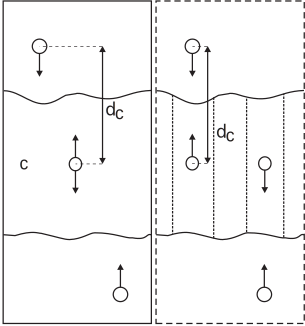
\includegraphics[width=6cm]{plots/pullref}}
\caption{Overview of the different reference group possibilities,
applied to interface systems. C is the reference group. The circles
represent the center of mass of 2 groups plus the reference group, and
$d_c$ is the reference distance.}
\label{fi:pullref} 
\end{figure}   

\begin{description}
\item[\tt com]\mbox{}\\ The center of mass of the group given under {\tt
reference\_group}, calculated each step from the current coordinates. 
\item[\tt com\_t0]\mbox{}\\ The center of mass of the group given under {\tt
reference\_group}, calculated each step from the current coordinates,
but corrected for atoms that have crossed the box. If the reference
group consists of all the water molecules in the system, and a single
water molecule moves across the box and enters from the other side,
the c.o.m. will show a slight jump. This is simply due to the periodic
boundary conditions, and shows that the center of mass in a simulation
in periodic boundary conditions is ill defined if the group
used to calculate it is \emph{e.g.} a slab of liquid. If the 'real'
positions are used instead of the coordinates that have been reset to
be inside the box, the center of mass of the \textbf{whole} system is 
conserved. 
\item[\tt dynamic]\mbox{}\\ In a phospholipid bilayer system it may be of
interest to calculate the pmf of a lipid as function of its distance
from the whole bilayer. The whole bilayer can be taken as reference
group in that case, but it might also be of interest to define the
reaction coordinate for the pmf more locally. {\tt dynamic} does not
use all the atoms of the {\tt reference\_group}, but instead only those
within a cylinder with radius {\tt r} below the main group. This only
works for distances defined in 1 dimension, and the cylinder is
oriented with its long axis along this 1 dimension. A second cylinder
can be defined with {\tt rc}, with a linear switch function that weighs
the contribution of atoms between {\tt r} and {\tt rc} with
distance. This smoothes the effects of atoms moving in and out of the
cylinder (which causes jumps in the constraint forces). 
\item[\tt dynamic\_t0]\mbox{}\\
The same as {\tt dynamic}, but the coordinates are corrected for
boxcrossings like in {\tt com\_t0}. Note that strictly speaking this is
not correct if the reference group is not the whole system, including
the groups defined with {\tt group\_1} and {\tt group\_2}.
\end{description}

To further smooth rapidly fluctuating distances between the reference
group and the other groups, the average distance can be constrained
instead of the instanteneous distance. This is defined by setting {\tt
reflag} to the number of steps to average over. However, using this
option is not strictly correct for calculating potentials of mean
force from the average constraint force. 

\subsubsection{The parameter file}

\begin{description}
\item[\tt verbose                  = no]\mbox{}\\
If this is set to {\tt yes}, a large amount of detailed information
is sent to {\tt stderr}, which is only useful for diagnostic
purposes. The {\tt .pdo} file also becomes more detailed, which is not
necessary for normal use.

\item[\tt runtype                  = constraint]\mbox{}\\
Options are {\tt start, afm, constraint, umbrella}. This selects the
type of calculation: making starting structures, AFM pulling,
constraint force calculation or umbrella sampling.

\item[\tt group\_1                  = MB21\_1]
\item[\tt group\_2                  = MB21\_2]\mbox{}\\                 
The groups with the atoms to act on. The first group is mandatory, the
second optional.

\item[\tt reference\_group          = OCTA]\mbox{}\\
The reference group. Distances are calculated betweeen {\tt group\_1}
(and {\tt group\_2} if specified) and this group. If \emph{e.g.} the
constraint force between two ions is needed, you would specifiy {\tt
group\_1} as a group with 1 ion, and {\tt reference\_group} as the other
ion.

\item[\tt reftype                  = com]\mbox{}\\
The type of reference group. Options are {\tt com, com\_t0, dynamic,
dynamic\_t0} as explained above. 

\item[\tt reflag                   = 1]\mbox{}\\
The position of the reference group can be taken as average over a
number of steps, specified by {\tt reflag} (see above).

\item[\tt direction                = 0.0 0.0 1.0]\mbox{}\\
Distances are calculated weighted by x, y, z as specified in {\tt
direction}. Setting them all to 1.0 calculates the distance between
two groups, setting the first two to 0.0 and the third to 1.0
calculates the distance in the z direction only.

\item[\tt reverse                  = to\_reference]\mbox{}\\
This option selects the direction in which the groups are moved with
respect to the reference group for AFM pull\-ing and start\-ing structure
calcu\-lations. Choices are {\tt to\_reference, from\_reference}.

\item[\tt r                        = 0]\mbox{}\\
If dynamic reference groups are selected ({\tt dynamic, dynamic\_t0}),
{\tt r} is the radius of the cylinder used to define which atoms are
part of the reference group (see above).

\item[\tt rc                       = 0]\mbox{}\\
With dynamic reference groups, the cylinder can be smoothly switched
so that atoms that fall between {\tt r} and {\tt rc} are weighted
linearly from 1 to 0 going from {\tt r} to {\tt rc}. As reasonable
initial values we suggest {\tt r = 1.0} and {\tt rc = 1.5} but this
will depend strongly on the exact system of interest.

\item[\tt update                   = 1]\mbox{}\\
The frequency with which the dynamic reference groups are
recalculated. Usually there is no reason to use anything other than 1.

\item[\tt pullrate                 = 0.00005]\mbox{}\\
The pull rate in nm/timestep for AFM pulling.

\item[\tt forceconstant            = 100]\mbox{}\\
The force constant for the spring in AFM pulling, in kJ mol$^{-1}$
nm$^{-2}$.

\item[\tt width                    = 0]\mbox{}\\
Width of the umbrella sampling potential in kJ mol$^{-1}$ nm$^{-2}$. 

\item[\tt r0\_group2                = 0.0  0.0   3.300]\mbox{}\\
The initial location of the groups with respect to the reference
group. Only coordinates selected with {\tt direction} are taken into account.
The groups are moved to these initial positions before the
actual creation of a series of starting structures commences.

\item[\tt tolerance                = 0.001]\mbox{}\\
The accuracy with which the actual position of the groups must match
the calculated ideal positions for a starting structure (in nm).
 
\item[\tt translation\_rate         = 0.00001]\mbox{}\\
The rate of translation in all directions (nm/step). As mentioned
above, normal MD force calculations and position updates also act on
the groups.

\item[\tt transstep                = 0.2]\mbox{}\\
The interval in nm at which structures are written out. 

\end{description}

\subsection{Output}
The output file is a text file with forces or positions, one per
line. If there are two groups they alternate in the output
file. Currently there is no supported analysis program to read this
file, but it is simple to parse.

\subsection{Limitations}
Apart from obvious limitations that are simply not implemented (\emph{e.g.} a
better umbrella sampling and analysis scheme), there is one important
limitation: constraint forces can \textbf{only} be calculated between
molecules or groups of molecules. If a group contains part of a
molecule of which the bondlengths are constrained, SHAKE or LINCS and
the constraint force calculation here will interfere with each other,
making the results unreliable. If a constraint force is wanted between
two atoms, this can be done through the free energy perturbation
code. In summary: 

\begin{itemize}
\item{\bf pull code:} between molecules or groups of molecules.
\item{\bf free energy perturbation code:} between single atoms. 
\item{\bf not possible currently:} between groups of atoms that are
part of a larger molecule for which the bonds are constrained with
SHAKE or LINCS.
\end{itemize}

\subsection{Implementation}

The code for the options described above can be found in the files
{\tt pull.c, pullinit.c, pullio.c, pullutil.c} and the headerfiles
{\tt pull.h} and {\tt pulls.h}. This last file defines a few
datatypes, {\tt pull.h} explains the main functions. 

\subsection{Future development}
There are several additional features that would be useful, including
more advanced umbrella sampling, an analysis tool to analyse the
output of the pull code, incorporation of the input parameters and
index file into the {\tt grompp} program input files, extension to more
groups, more flexible definition of a reaction coordinate, extension
to groups that are parts of molecules that use SHAKE or LINCS, and a
combination of the starting structure calculation with constraints for
faster convergence of starting structures.


%%%%%%%%%%%%%%%%%%%%%%%%%%%%%%%%%%%%%%%%%%%%%%%%%%%%%%%%%%%%%%%%%%%%%%%%%%%%%%%
%%%%%%%%%%%%%%%%%%%%%%%%%%%%%%%%%%%%%%%%%%%%%%%%%%%%%%%%%%%%%%%%%%%%%%%%%%%%%%%
%%%%%%%%%%%%%%%%%%%%%%%%%%%%%%%%%%%%%%%%%%%%%%%%%%%%%%%%%%%%%%%%%%%%%%%%%%%%%%%
\newcommand{\amine}{\sf -NH$_2$}
\newcommand{\amines}{\sf -NH-}
\newcommand{\aminep}{\sf -NH$_3^+$}
\section{Removing fastest \swapindex{degrees of}{freedom}}
The maximum time step in MD simulations is limited by the smallest
oscillation period that can be found in the simulated
system. Bond-stretching vibrations are in their quantum-mechanical
ground state and are therefore better represented by a constraint than
by a harmonic potential.

For the remaining degrees of freedom, the shortest oscillation period
as measured from a simulation is 13~fs for bond-angle vibrations
involving hydrogen atoms. Taking as a guideline that with a Verlet
(leap-frog) integration scheme a minimum of 5 numerical integration
steps should be performed per period of a harmonic oscillation in
order to integrate it with reasonable accuracy, the maximum time step
will be about 3~fs. Disregarding these very fast oscillations of
period 13~fs the next shortest periods are around 20~fs, which will
allow a maximum time step of about 4~fs

Removing the bond-angle degrees of freedom from hydrogen atoms can
best be done by defining them as \swapindex{dummy}{atom}s in stead of
normal atoms. Where a normal atoms is connected to the molecule with
bonds, angles and dihedrals, a dummy atom's position is calculated
from the position of three nearby heavy atoms in a predefined manner
(see also \secref{dummy}). For the hydrogens in water and in
hydroxyl, sulfhydryl or amine groups, no degrees of freedom can be
removed, because rotational freedom should be preserved. The only
other option available to slow down these motions, is to increase the
mass of the hydrogen atoms at the expense of the mass of the connected
heavy atom. This will increase the moment of inertia of the water
molecules and the hydroxyl, sulfhydryl or amine groups, without
affecting the equilibrium properties of the system and without
affecting the dynamical properties too much. These constructions will
shortly be described in \secref{dummyhydro} and have previously
been described in full detail~\cite{feenstra99}.

Using both dummy atoms and \swapindex{modified}{mass}es, the next
bottleneck is likely to be formed by the improper dihedrals (which are
used to preserve planarity or chirality of molecular groups) and the
peptide dihedrals. The peptide dihedral cannot be changed without
affecting the physical behavior of the protein. The improper dihedrals
that preserve planarity, mostly deal with aromatic residues. Bonds,
angles and dihedrals in these residues can also be replaced with
somewhat elaborate dummy atom constructions, as will be described in
\secref{dummyaro}~\cite{feenstra01}.

All modifications described in this section can be performed using the
{\gromacs} topology building tool {\tt \normindex{pdb2gmx}}. Separate
options exist to increase hydrogen masses, dummify all hydrogen atoms
or also dummify all aromatic residues. Note that when all hydrogen
atoms are dummified, also those inside the aromatic residues will be
dummified, {\ie} hydrogens in the aromatic residues are treated
differently depending on the treatment of the aromatic residues.

Parameters for the dummy constructions for the hydrogen atoms are
inferred from the forcefield parameters ({\em vis}. bond lengths and
angles) directly by {\tt \normindex{grompp}} while processing the
topology file.  The constructions for the aromatic residues are based
on the bond lengths and angles for the geometry as described in the
forcefields, but these parameters are hard-coded into {\tt
\normindex{pdb2gmx}} due to the complex nature of the construction
needed for a whole aromatic group.

\subsection{Hydrogen bond-angle vibrations}
\label{sec:dummyhydro}
\subsubsection{Construction of Dummy Atoms} %%%%%%%%%%%%%%%%%%%%%%%%%
\begin{figure}
\centerline{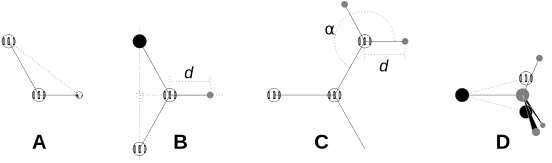
\includegraphics[width=11cm]{plots/dumtypes}}
\caption[Dummy atom constructions for hydrogen atoms.]{The different
types of dummy atom constructions used for hydrogen atoms. The atoms
used in the construction of the dummy atom(s) are depicted as black
circles, dummy atoms as grey ones. Hydrogens are smaller than heavy
atoms. {\sf A}: fixed bond angle, note that here the hydrogen is not a
dummy atom; {\sf B}: in the plane of three atoms, with fixed distance;
{\sf C}: in the plane of three atoms, with fixed angle and distance;
{\sf D}: construction for amine groups ({\amine} or {\aminep}), see
text for details.}
\label{fig:dumhydro}
\end{figure}

The goal of defining hydrogen atoms as dummy atoms is to remove all
high-frequency degrees of freedom from them. In some cases not all
degrees of freedom of a hydrogen atom should be removed, {\eg} in the
case of hydroxyl or amine groups the rotational freedom of the
hydrogen atom(s) should be preserved. Care should be taken that no
unwanted correlations are introduced by the construction of dummy
atoms, {\eg} bond-angle vibration between the constructing atoms could
translate into hydrogen bond-length vibration. Additionally, since
dummy atoms are by definition mass-less, in order to preserve total
system mass, the mass of each hydrogen atom that is treated as dummy
atom should be added to the bonded heavy atom.

Taking into account these considerations, the hydrogen atoms in a
protein naturally fall into several categories, each requiring a
different approach, see also \figref{dumhydro}:

\begin{itemize}

\item{\em hydroxyl ({\sf -OH}) or sulfhydryl ({\sf -SH})
hydrogen:\/} The only internal degree of freedom in a hydroxyl group
that can be constrained is the bending of the {\sf C-O-H} angle. This
angle is fixed by defining an additional bond of appropriate length,
see \figref{dumhydro}A. This removes the high frequency angle bending,
but leaves the dihedral rotational freedom. The same goes for a
sulfhydryl group. Note that in these cases the hydrogen is not treated
as a dummy atom.

\item{\em single amine or amide ({\amines}) and aromatic hydrogens
({\sf -CH-}):\/} The position of these hydrogens cannot be constructed
from a linear combination of bond vectors, because of the flexibility
of the angle between the heavy atoms. In stead, the hydrogen atom is
positioned at a fixed distance from the bonded heavy atom on a line
going through the bonded heavy atom and a point on the line through
both second bonded atoms, see \figref{dumhydro}B.

\item{\em planar amine ({\amine}) hydrogens:\/} The method used for
the single amide hydrogen is not well suited for planar amine groups,
because no suitable two heavy atoms can be found to define the
direction of the hydrogen atoms. In stead, the hydrogen is constructed
at a fixed distance from the nitrogen atom, with a fixed angle to the
carbon atom, in the plane defined by one of the other heavy atoms, see
\figref{dumhydro}C.

\item{\em amine group (umbrella {\amine} or {\aminep}) hydrogens:\/}
Amine hydrogens with rotational freedom cannot be constructed as dummy
atoms from the heavy atoms they are connected to, since this would
result in loss of the rotational freedom of the amine group. To
preserve the rotational freedom while removing the hydrogen bond-angle
degrees of freedom, two ``dummy masses'' are constructed with the same
total mass, moment of inertia (for rotation around the {\sf C-N} bond)
and center of mass as the amine group. These dummy masses have no
interaction with any other atom, except for the fact that they are
connected to the carbon and to each other, resulting in a rigid
triangle. From these three particles the positions of the nitrogen and
hydrogen atoms are constructed as linear combinations of the two
carbon-mass vectors and their outer product, resulting in an amine
group with rotational freedom intact, but without other internal
degrees of freedom. See \figref{dumhydro}D.

\end{itemize}

\begin{figure}
\centerline{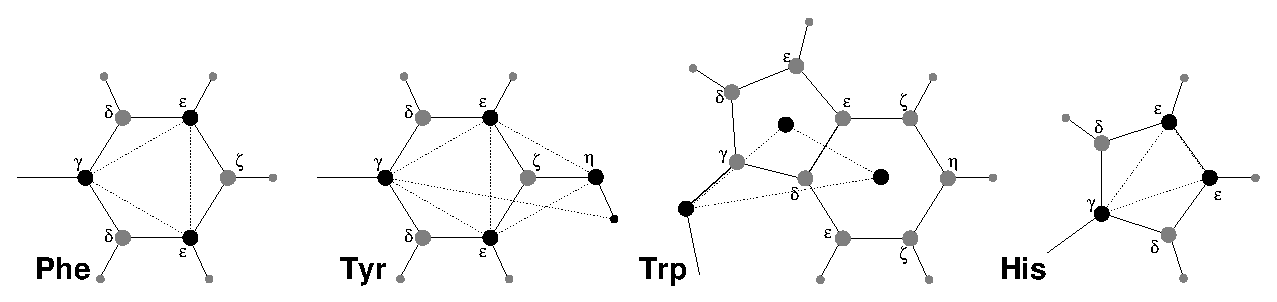
\includegraphics[width=15cm]{plots/dumaro}}
\caption[Dummy atom constructions for aromatic residues.]{The
different types of dummy atom constructions used for aromatic
residues. The atoms used in the construction of the dummy atom(s) are
depicted as black circles, dummy atoms as grey ones. Hydrogens are
smaller than heavy atoms. {\sf A}: phenylalanine; {\sf B}: tyrosine
(note that the hydroxyl hydrogen is {\em not} a dummy atom); {\sf C}:
tryptophane; {\sf D}: histidine.}
\label{fig:dumaro}
\end{figure}

\subsection{Out-of-plane vibrations in aromatic groups}
\label{sec:dummyaro}
The planar arrangements in the side chains of the aromatic residues
lends itself perfectly for a dummy-atom construction, giving a
perfectly planar group without the inherently instable constraints
that are necessary to keep normal atoms in a plane. The basic approach
is to define three atoms or dummy masses with constraints between them
to fix the geometry and create the rest of the atoms as simple dummy
type 3 atoms (see \secref{dummy}) from these three. Each of
the aromatic residues require a different approach:

\begin{itemize}

\item{\em Phenylalanine:\/} {\sf C}$_\gamma$, {\sf C}$_{{\epsilon}1}$
and {\sf C}$_{{\epsilon}2}$ are kept as normal atoms, but with each a
mass of one third the total mass of the phenyl group. See
\figref{dumhydro}A.

\item{\em Tyrosine:\/} The ring is treated identical to the
phenylalanine ring. Additionally, constraints are defined between {\sf
C}$_{{\epsilon}1}$ and {\sf C}$_{{\epsilon}2}$ and {\sf O}$_{\eta}$.
The original improper dihedral angles will keep both triangles (one
for the ring and one with {\sf O}$_{\eta}$) in a plane, but due to the
larger moments of inertia this construction will be much more
stable. The bond angle in the hydroxyl group will be constrained by a
constraint between {\sf C}$_\gamma$ and {\sf H}$_{\eta}$, note that
the hydrogen is not treated as a dummy atom. See
\figref{dumhydro}B.

\item{\em Tryptophane:\/} {\sf C}$_\beta$ is kept as a normal atom
and two dummy masses are created at the center of mass of each of the
rings, each with a mass equal to the total mass of the respective ring
({\sf C}$_{{\delta}2}$ and {\sf C}$_{{\epsilon}2}$ are each
counted half for each ring). This keeps the overall center of mass and
the moment of inertia almost (but not quite) equal to what it was. See
\figref{dumhydro}C.

\item{\em Histidine:\/} {\sf C}$_\gamma$, {\sf C}$_{{\epsilon}1}$
and {\sf N}$_{{\epsilon}2}$ are kept as normal atoms, but with masses
redistributed such that the center of mass of the ring is
preserved. See \figref{dumhydro}D.

\end{itemize}

\section{\normindex{Viscosity} calculation}

The shear viscosity is a property of liquid which can be determined easily  
by experiment. It is useful for parameterizing the forcefield,
because it is a kinetic property, while most other properties
which are used for parameterization are thermodynamic.
The viscosity is also an important property, since it is of influence on
the rates of conformational changes of molecules solvated in the liquid.

The viscosity can be calculated from an equilibrium simulation using
an Einstein relation:
\beq
\eta = \frac{1}{2}\frac{V}{k_B T} \lim_{t \rightarrow \infty}
\frac{\mbox{d}}{\mbox{d} t} \left\langle 
\left( \int_{t_0}^{{t_0}+t} P_{xz}(t') \mbox{d} t' \right)^2
\right\rangle_{t_0}
\eeq
This can be done with {\tt g\_energy}.
This method converges very slowly. A nanosecond simulation might not
be long enough for an accurate determinination of the viscoity.
The result is very dependent on the treatment of the electrostatics.
Using a (short) cut-off results in large noise on the off-diagonal
pressure elements, which can increase the calculated viscosity by an order
of magnitude.

{\gromacs} also has a non-equilibrium method for determining the viscosity.
This makes use of the fact that energy, which is fed into system by
external forces, is dissipated through viscous friction. The generated heat
is removed by coupling to a heat bath. For a Newtonian liquid adding a 
small force will result in a velocity gradient according to the following
equation:
\beq
a_x(z) + \frac{\eta}{\rho} \frac{\partial^2 v_x(z)}{\partial z^2} = 0
\eeq
here we have applied an acceleration $a_x(z)$ in the $x$-direction, which
is a function of the $z$-coordinate.
In {\gromacs} the acceleration profile is:
\beq
a_x(z) = A \cos\left(\frac{2\pi z}{l_z}\right)
\eeq
where $l_z$ is the height of the box. The generated velocity profile is:
\beq
v_x(z) = V \cos\left(\frac{2\pi z}{l_z}\right)
\eeq
\beq
V = A \frac{\rho}{\eta}\left(\frac{l_z}{2\pi}\right)^2
\eeq
The viscosity can be calculated from $A$ and $V$:
\beq
\label{visc}
\eta = \frac{A}{V}\rho \left(\frac{l_z}{2\pi}\right)^2
\eeq

In the simulation $V$ is defined as:
\beq
V = \frac{\displaystyle \sum_{i=1}^N m_i v_{i,x} 2 \cos\left(\frac{2\pi z}{l_z}\right)}
         {\displaystyle \sum_{i=1}^N m_i}
\eeq
The generated velocity profile is not coupled to the heat bath, also
the velocity profile is excluded from the kinetic energy.
One would like $V$ to be as large as possible to get good statistics.
However the shear rate should not be so high that the system gets too far
from equilibrium. The maximum shear rate occurs where the cosine is zero,
the rate is:
\beq
\mbox{sh}_{\max} =  \max_z \left| \frac{\partial v_x(z)}{\partial z} \right|
= A \frac{\rho}{\eta} \frac{l_z}{2\pi}
\eeq
For a simulation with: $\eta=10^{-3}$ [kg\,m$^{-1}$\,s$^{-1}$],
$\rho=10^3$\,[kg\,m$^{-3}$] and $l_z=2\pi$\,[nm],
$\mbox{sh}_{\max}=1$\,[ps\,nm$^{-1}$] $A$.
This shear rate should be smaller than one over the longest
correlation time in the system. For most liquids this will be the rotation
correlation time, which is around 10 picoseconds. In this case $A$ should
be smaller than 0.1\,[nm\,ps$^{-2}$].
When the shear rate is too high, the observed viscosity will be too low.
Because $V$ is proportional to the square of the box height,
the optimal box is elongated in the $z$-direction.
In general a simulation length of 100 picoseconds is enough to obtain an
accurate value for the viscosity.

The heat generated by the viscous friction is removed by coupling to a heat
bath. Because this coupling is not instantaneous the real temperature of the
liquid will be slightly lower than the observed temperature.
Berendsen derived this temperature shift\cite{Berendsen91}{,} which can
be written in terms of the shear rate as:
\beq
T_s = \frac{\eta\,\tau}{2 \rho\,C_v} \mbox{sh}_{\max}^2
\eeq
where $\tau$ is the coupling time for the Berendsen thermostat and
$C_v$ is the heat capacity. Using the values of the example above,
$\tau=10^{-13}$ [s] and $C_v=2 \cdot 10^3$\,[J kg$^{-1}$\,K$^{-1}$], we
get: $T_s=25$\,[K\,ps$^{-2}$]\,sh$_{\max}^2$. When we want the shear
rate to be smaller than $1/10$\,[ps$^{-1}$], $T_s$ is smaller than
0.25\,[K], which is negligible.

Note that the system has to build up the velocity profile when starting
from an equilibrium state. This build-up time is of the order of the
correlation time of the liquid.

Two quantities are written to the energy file, along with their averages
and fluctuations: $V$ and $1/\eta$ as obtained from (\ref{visc}).

\section{User specified potential functions}
You can also use your own \swapindex{potential}{function}s 
without editing the {\gromacs} code. 
The potential function should be according to the following equation
\beq
V(r_{ij}) ~=~ \frac{q_i q_j}{4 \pi\epsilon_0} f(r_{ij}) + C_6 g(r_{ij}) + C_{12} h(r_{ij})
\eeq
with f,g,h user defined functions. Note that if g(r) represents a
normal dispersion interaction, g(r) should be $<$ 0. C$_6$, C$_{12}$
and the charges are read from the topology. Also note that combination
rules are only supported for Lennard Jones and Buckingham, and that
your tables should match the parameters in the binary topology.

When you add the following lines in your {\tt .mdp} file:
\begin{verbatim}
rlist           = 1.0
coulombtype     = User
rcoulomb        = 1.0
vdwtype         = User
rvdw            = 1.0
\end{verbatim}
the MD program will read a single file (name can be changed with
option {\tt -table}) with seven columns of table lookup data in the
order: x, f(x), f''(x), g(x), g''(x), h(x), h''(x).  The x should run
from 0 to r$_c$+0.5, with a spacing of 0.002 nm when you run in single
precision, or 0.0005 when you run in double precision.  In this
context r$_c$ denotes the maximum of the two cut-offs {\tt rvdw} and
{\tt rcoulomb} (see above). These variables need not be the same (and
need not be 1.0 either).  Some functions used for potentials contain a
singularity at x = 0, but since atoms are normally not closer to each
other than 0.1 nm, the function value at x = 0 is not important and
the tables can be started at e.g. 0.02 nm.  Finally, it is also
possible to combine a standard Coulomb with a modified LJ potential
(or vice versa). One then specifies e.g. coulombtype = Cut-off or
coulombtype = PME, combined with vdwtype = User.  The table file must
always contain the 7 columns however, and meaningful data (i.e. not
zeroes) must be entered in all columns.  A number of pre-built table
files can be found in the GMXLIB directory, for 6-8, 6-9, 6-10, 6-11, 6-12
Lennard Jones potentials combined with a normal Coulomb.


\section{Running {\gromacs} in parallel}
If you have installed the MPI (Message Passing Interface) on your computer(s)
you can compile {\gromacs} with this library to run simulations in parallel. 
All supercomputers are shipped with MPI libraries optimized for 
that particular platform, and if you are using a cluster of workstations
there are several good free MPI implementations. You can find updated links
to these on the gromacs homepage {\wwwpage}. Once you have an MPI library
installed it's trivial to compile {\gromacs} with MPI support: Just set
the option {\tt --enable-mpi} to the configure script and recompile.
(But don't forget to make distclean before running configure if you have
previously compiled with a different configuration.) If you are using a 
supercomputer you might also want to turn of the default nicing of the
mdrun process with the {\tt --disable-nice} option.

There is usually a program called {\tt mpirun} with which you can fire
up the parallel processes. A typical command line looks like:
\type{mpirun -p goofus,doofus,fred 10 mdrun -s topol -v -N 30}
this runs on each of the machines goofus,doofus,fred with 10 processes
on each\footnote{Example taken from Silicon Graphics manual}.

If you have a single machine with multiple processors you don't have to
use the {\tt mpirun} command, but you can do with an extra option to
{\tt mdrun}:
\type{mdrun -np 8 -s topol -v -N 8}
In this example MPI reads the first option from the command line.
Since {\tt mdrun} also wants to know the number of processes you have to
type it twice.

Check your local manuals (or online manual) for exact details
of your MPI implementation.

If you are interested in programming MPI yourself, you can find
manuals and reference litterature on the web at
\href{http:://www.mcs.anl.gov/mpi/index.html}{www.mcs.anl.gov/mpi/index.html}.


